\chapter{Light Field Tomography}

\section{A Model for Light Attenuation}
%TODO: Derivation according to Wetzstein
% Explain linearity in log domain
% Mention other tomographic projection types
% SART and ART solvers
% Explain "intensity of ray" and unit

The light field display is modeled by a volumetric attenuator $\mu(x, y, z)$ that attenuates the light traveling through its material.
According to the Beer-Lambert law, the intensity of a light ray $\mathcal{R} \subset \mathbb{R}^3$ passing through the material decreases exponentially over distance:
\begin{equation}\label{eq:beer_lambert_law}
I = I_0 e^{-\int_\mathcal{R} \mu(r) \, \mathrm{d}r }.
\end{equation}
The incident intensity $I_0$ is the intensity of the ray before it enters the attenuator.
Equation~\ref{eq:beer_lambert_law} can be rewritten into 
\begin{equation}\label{eq:log_beer_lambert_law}
\bar{I} \coloneqq \log \left( \frac{I}{I_0} \right) = -\int_\mathcal{R} \mu(r) \, \mathrm{d}r.
\end{equation} 
Now, let the attenuator $\mu(x, y, z)$ be a cubic slab of height $d$ in Z-direction and let $L(u, v, s, t)$ be the two-plane parameterization of the light field such that the $(s, t)$-plane coincides with the $(x, y)$-plane of the attenuator and the $(u, v)$-plane is at distance $d$.
The set of points describing the ray defined by the coordinates $(u, v, s, t)$ is
\begin{equation}
\mathcal{R} = \left\{ \lambda a + b 
\mathrel{\bigg|} a = 
\begin{pmatrix}
u - s \\ 
v - t \\ 
d
\end{pmatrix}, 
b = 
\begin{pmatrix}
s \\ 
t \\ 
0
\end{pmatrix},
\lambda \in \mathbb{R} 
\right\}.
\end{equation}
A point $p = (x, y, z)^T$ is part of the ray $\mathcal{R}$ if and only if
\begin{align}
& \exists \lambda \in \mathbb{R} : p = \lambda a + b & & \iff & & a \times (p - b) = 0, 
\end{align} 
where $\times$ denotes the cross product.
Now, $I$ can be replaced with the light field $L$ and the right hand side of equation~\ref{eq:log_beer_lambert_law} can be written as an integral over~$\mathbb{R}^3$:
\begin{equation}\label{eq:log_lightfield_and_radon_transform}
\bar{L}(u, v, s, t) = 	%\int \limits_{-\infty}^{\infty} \int \limits_{-\infty}^{\infty} \int \limits_{-\infty}^{\infty}
-\int_{\mathbb{R}^3}
\mu(p) \delta ( a \times (p - b) ) \, 
\mathrm{d}p.
\end{equation}
Here, $\delta$ denotes the Dirac delta function on $\mathbb{R}^3$ and $\mu$ is zero outside the boundaries of the slab. 
This means that the integrand is only non-zero for points on the ray with coordinates $(u, v, s, t)$.

Combining equation~\ref{eq:beer_lambert_law} and~\ref{eq:log_lightfield_and_radon_transform} gives the light field emitted by the attenuator.
The goal is to produce such an attenuation display that emits a given target light field.

In computed tomography, the \textbf{Radon transform} of a real valued and compactly supported, continuous function $f(x, y)$ on $\mathbb{R}^2$ is defined as
\begin{equation}
p(\rho, \theta) = 	\int \limits_{-\infty}^{\infty} 
\int \limits_{-\infty}^{\infty}
f(x, y) \delta (x \cos \theta - y \sin \theta - \rho) \, 
\mathrm{d}x \,
\mathrm{d}y,
\end{equation}
where $(\rho, \theta) \in \mathbb{R} \times \left(- \frac{\pi}{2}, \frac{\pi}{2}\right)$ defines a ray as shown in figure~\ref{fig:radon_transform_2D_sketch}.
Because the Radon transform is essentially a line integral, it can be generalized to three or more dimensions.
\begin{figure}[tb]
	\centering
	\documentclass{standalone}
\usepackage{tikz}
\usetikzlibrary{intersections}

\begin{document}
	
	\begin{tikzpicture}[scale = 0.5]
		
		\draw[->] (-5, 0) -- (5, 0);
		\draw[->] (0, -5) -- (0, 5);
		\node[right] at (5, 0) {$x$};
		\node[above] at (0, 5) {$y$};
		
		\draw plot[smooth cycle] coordinates {(-3, 1) (-2, 2.5) (0, 2) (1.5, 3.5) (2, 2) (2.5, 1) (2, 0) (2, -2) (0.5, -1.5) (-2, -3) (-2, -1)};
		
		\draw[<-] (-1.5, 7.5) -- (-7.5, -1.5); %node[below right] {$\rho$};
		
		\draw[name path = ray, ->] (4, -0.5) -- (-6.5, 6.5);
		\draw (0, 0) -- (-7.5, 5);
		
		\draw (0, 1.5) arc (90 : 180 - atan(2 / 3) : 1.5);
		\node at (-0.4, 0.8) {$\theta$};
		
		\draw[->] (0, 0) -- (1, 1.5) node[pos = 0.4, right] {$\rho$};
		
		\draw[name path = radon] plot[smooth] coordinates {(-6.5, 0) (-6.7, 0.5) (-6.5, 1.2) (-6, 2) (-6.5, 3) (-6, 4.5) (-5, 4.5) (-4, 5.5) (-2.5, 6)};
		
		\fill[name intersections={of= radon and ray, total=\t}]
		\foreach \s in {1,...,\t}{(intersection-\s) circle[radius = 0.1] node[rotate= 90 - atan(2 / 3), above right] {$p(\rho, \theta)$}};
		
		\node[rotate= 90 - atan(2 / 3), right] at (-1.5, 7.5) {$\rho$};
		
	\end{tikzpicture}
	
\end{document}
	\caption{The 2D Radon transform of the ray $(\rho, \theta)$ passing a material with density $f(x, y)$.}
	\label{fig:radon_transform_2D_sketch}
\end{figure}
Adapting the notation from the two-plane parameterization, the Radon transform of the attenuation map $\mu$ along ray $\mathcal{R}$ becomes
\begin{equation}
p(u, v, s, t) = 	\int \limits_{-\infty}^{\infty} 
\int \limits_{-\infty}^{\infty}
\int \limits_{-\infty}^{\infty}
\mu(x, y, z) \delta \left(a \times \left((x, y, z)^T - b\right) \right) \, 
\mathrm{d}x \,
\mathrm{d}y \,
\mathrm{d}z, 
\end{equation}
which is equivalent to equation~\ref{eq:log_lightfield_and_radon_transform}.
This shows that
\begin{equation}\label{eq:log_light_field_negative_radon}
\bar{L}(u, v, s, t) = -p(u, v, s, t), 
\end{equation}
or with the words of~\cite{WetzsteinTomo}: \say{The logarithm of the emitted light field is equivalent to the negative Radon transform of the attenuation map.}

\section{Discrete Attenuation Layers}

The previous section introduced a continuously varying attenuation map to model the display.
\cite{WetzsteinTomo} propose to represent the attenuator with a set of $N$ two-dimensional layers, also called masks.

Let $L_{ijkl} = L(u(i), v(j), s(k), t(l))$ be the matrix of samples from the light field and for simplicity, let $m \coloneqq m(i, j, k, l)$ be a linear index of the 4D indices.
Equation \ref{eq:beer_lambert_law} suggests a per-ray constraint in the form
\begin{equation}\label{eq:transmittance_layers}
	L_m = L_0 \prod_{n=1}^{N} t^{(n)} (h(m, n)), 
\end{equation}
where $h(m, n)$ is the (discrete) 2D coordinate of the intersection of the \mbox{$m$-th} ray with the \mbox{$n$-th} layer, and $t^{(n)}(\xi)$ is the \textbf{transmittance} of layer $n$ at that coordinate.
Having a constraint for each ray, the goal is to solve for the transmittance~$t$.
However, the system of equations in~\ref{eq:transmittance_layers} is non-linear and cannot directly be solved.
One can obtain a linear system of equations by taking the logarithm in~\ref{eq:transmittance_layers}:
\begin{equation}\label{eq:discrete_log_light_field_negative_radon}
	\bar{L}_m 	=	\sum_{n = 1}^{N}
					\log \left( t^{(n)} (h(m, n)) \right) 
				= 	-\sum_{n = 1}^{N} a^{(n)} (h(m, n)) 
				= -P_m \alpha.
\end{equation}
Here, $a^{(n)} \coloneqq -\log t^{(n)}$ denotes the \textbf{absorbance} of layer $n$. 
This relation between transmittance and absorbance also directly follows from the Beer-Lambert law.
Here, $P_m = \left( P_m^{(1)}, \dots, P_m^{(N)} \right)$ is a binary row vector, encoding the intersection of the ray with the pixels on each layer.
The unknown absorbance is represented by the column vector $\alpha = \left( \alpha^{(1)}, \dots, \alpha^{(N)} \right)^T$.
Each $\alpha^{(i)}$ is just a flattened representation of the absorbance matrix $a^{(i)}$.
Note that equation~\ref{eq:discrete_log_light_field_negative_radon} is the equivalent of the continuous version in~\ref{eq:log_light_field_negative_radon}, since $P_m$ encodes the Radon transform.
Finally, the above equations indexed by $m$ can be combined into one large linear system $P \alpha = -\bar{L}$.

In most cases, $P$ is not a square matrix and the system can become overdetermined, which means that it has no solution in general.
However, it is still possible to find values for $\alpha$ such that the error $\left\lVert P \alpha + \bar{L} \right\rVert$ is small. 
Thus, the objective becomes
\begin{equation} \label{eq:minimize_norm}
	\begin{aligned}
		& \underset{\alpha}{\text{argmin}} 	& & \left\lVert P \alpha + \bar{L} \right\rVert ^2 \\
		& \text{subject to} 				& & 0 \leq \alpha \leq \infty.
	\end{aligned}
\end{equation}
Finally, when optimal values $\alpha$ are found, the transmittance used to fabricate the layers is obtained by calculating $e^{-\alpha}$.
Also note that the matrix P is very sparse because it is assumed that a ray passes through each layer at exactly one pixel no more than once and inter-reflections between the layers are not supported by the model.
Thus, $P$ can be efficiently stored using an appropriate data structure.

\section{Iterative Reconstruction}

%TODO: Show plot of residual norm in each iteration
%TODO: Compare to linear least squares method from MATLAB
%TODO: Mention choice of relaxation parameter lambda = 1

The optimization problem in equation~\ref{eq:minimize_norm} is essentially a fitting problem.
Theoretically, it can be solved in a least squares sense using the normal equation $P^T P \alpha = P^T \bar{L}$ and by inverting the matrix $P^T P$.
For high resolution light fields, the matrix $P$ becomes extremely large and it is unfeasible to compute the inverse of $P^T P$.

In general, the approach to solve these kind of problems is to use iterative methods.
The choice of the method depends on the type of problem and the structure of the design matrix.
In computed tomography, a variety of iterative solvers have been developed to solve the exact same problem. 
Among the different methods is the Simultaneous Algebraic Reconstruction Technique (\mbox{SART}) first proposed by \cite{SART}.
The update rule of \mbox{SART} for iteration $k = 0, 1, 2, \dots$ is
\begin{equation}\label{eq:SART_update_rule}
	\alpha^{(k + 1)} = \alpha^{(k)} + \lambda C P^T R \left( \bar{L} - P \alpha^{(k)} \right), 	
\end{equation}
where $\lambda$ is a relaxation factor.
$R$ and $C$ denote the diagonal matrices with entries $R_{ii} = \frac{1}{r_i}$ and $C_{ii} = \frac{1}{c_i}$, where $r_i$ and $c_i$ are the sum of the elements in the \mbox{$i$-th} row and column of $P$ respectively.
The parts in~\ref{eq:SART_update_rule} involving $P$ and $P^T$ are also referred to as the \textbf{forward}- and \textbf{back-projection} respectively.

The convergence of \mbox{SART} has been studied by \cite{ConvergenceSART2}.
They have proven that it converges to a weighted least squares solution.

\section{Ray Casting}
\label{sec:ray_casting}

To obtain the linear system $P$, the intersections between the rays and the attenuation layers have to be calculated.
This calculation depends on the parameterization of the light field.
For continuous light fields, it is always possible to apply a re-parameterization to get the desired representation (e.g. the two-plane parameterization) and then compute the intersection in a standard way.
For discrete light fields however, this would require a suitable interpolation in ray-space, which gives poor results when the distribution of samples in the target space becomes too sparse.

What follows is a description of two methods to compute the indices for the non-zero entries in $P$. 
For simplicity, a two-dimensional attenuator of size $w$ is assumed, consisting of $N$ layers at various depths 
$Z_{\text{min}} = z_1 < z_2 < \dots < z_N = Z_{\text{max}}$.
It is also assumed that the image plane $s$ of the virtual cameras is bisecting the attenuator in the middle, at depth 
$z_0 = \frac{Z_{\text{max}} - Z_{\text{min}}}{2}$.

\subsection*{Oblique Projection}

The setup for the oblique projection type is illustrated in figure~\ref{fig:ray_casting_oblique_projection}.
Let $\theta_i$ denote the angle of the \mbox{$i$-th} oblique view from the light field.
Following the notation in previous sections, the linear index $m = m(i, k)$ indentifies the ray $(\theta_i, s(k))$.
The intersection of ray $m$ with the \mbox{$n$-th} layer is simply
\begin{equation}\label{eq:layer_intersection}
	h(m, n) = s(k) + \Delta z \tan (\theta_i), 
\end{equation}
where $\Delta z = z_0 - z_n$ is the displacement of layer $n$ from the image plane.
The next step is to compute the pixel index at the point $h(m, n)$.
The shift in pixel units can directly be derived from the shift in equation~\ref{eq:layer_intersection} given the pixel size $\Delta s$, yielding
\begin{equation}
	\Delta k = \left[ \frac{\Delta z \tan (\theta_i)}{\Delta s} \right],
\end{equation}
and the new index is $k^\prime = k + \Delta k$.
The brackets in the above equation denote the rounding operation.
Finally, this information is stored in the propagation matrix with the assignment $P_{m k^\prime}^{(n)} = 1$.

\begin{figure}[htb]
	\centering
	\documentclass{standalone}
\usepackage{tikz}
\usepackage{xcolor}

\begin{document}
	
	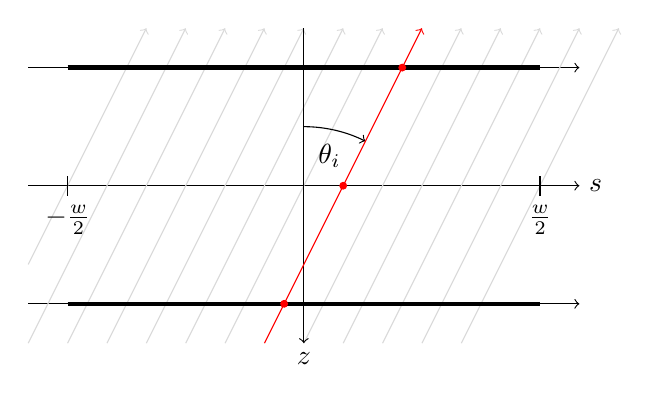
\begin{tikzpicture}[scale = 0.25]
	
		\colorlet{lightgray}{gray!30}
		
		% Top and bottom layer planes
		\draw[->] (-14, -6) -- (14, -6);
		\draw[->] (-14, 6) -- (14, 6);
		
		% Sensor plane
		\draw[<-] (14, 0) -- (-14, 0);
		\node[right] at (14, 0) {$s$};
		
		% Rays and intersections
		
		\draw[->, lightgray] (8, -8) -- (16, 8);
		\draw[->, lightgray] (6, -8) -- (14, 8);
		\draw[->, lightgray] (4, -8) -- (12, 8);
		\draw[->, lightgray] (2, -8) -- (10, 8);
		\draw[->, lightgray] (0, -8) -- (8, 8);
		
		\draw[->, lightgray] (-4, -8) -- (4, 8);
		\draw[->, lightgray] (-6, -8) -- (2, 8);
		\draw[->, lightgray] (-8, -8) -- (0, 8);
		\draw[->, lightgray] (-10, -8) -- (-2, 8);
		\draw[->, lightgray] (-12, -8) -- (-4, 8);
		\draw[->, lightgray] (-14, -8) -- (-6, 8);
		\draw[->, lightgray] (-14, -4) -- (-8, 8);
		
		\draw[ultra thick] (-12, -6) -- (12, -6);
		\draw[ultra thick] (-12, 6) -- (12, 6);
		
		% z-axis
		\draw[->] (0, 8) -- (0, -8);
		\node[below] at (0, -8) {$z$};
		
		% Angle and label
		\draw[->] (0, 3) arc (90 : atan(2) : 7);
		\node at (1.3, 1.5) {$\theta_i$};
		
		% Draw red ray on top of everything
		\draw[->, red] (-2, -8) -- (6, 8);	
		
		% Intersection markers
		\fill[red] (2, 0) circle[radius = 0.2];
		\fill[red] (5, 6) circle[radius = 0.2];
		\fill[red] (-1, -6) circle[radius = 0.2];	
		
		% Width markers
		\draw (-12, -0.5) -- (-12, 0.5);
		\draw (12, -0.5) -- (12, 0.5);
		\node[below] at (-12, -0.5) {$-\frac{w}{2}$};
		\node[below] at (12, -0.5) {$\frac{w}{2}$};
		
	\end{tikzpicture}
	
\end{document}
	\caption{Computation of the ray-layer intersection for the construction of the propagation matrix.
			 Two attenuation layers are drawn (top and bottom) with the virtual image plane in the center.
			 Light rays (gray) at a fixed angle $\theta_i$ intersect the layers at positions to be calculated.}
	\label{fig:ray_casting_oblique_projection}
\end{figure}

\subsection*{Perspective Projection}

\begin{figure}[htb]
	\centering
	\documentclass{standalone}
\usepackage{tikz}
\usepackage{xcolor}
\usetikzlibrary{intersections}

\begin{document}
	
	\begin{tikzpicture}[scale = 0.25,
						one end extended/.style={shorten <=-#1},
	 					one end extended/.default=1cm,
	 					]
	
		\colorlet{lightgray}{gray!30}
		
		% Top and bottom layer planes
		\draw[->, name path = bottomLayer] (-14, -6) -- (14, -6);
		\draw[->, name path = topLayer] (-14, 6) -- (14, 6);
					
		% Camera plane
		\draw[->] (-14, 15) -- (14, 15);
		\node[right] at (14, 15) {$u$};
		
		% Sensor plane
		\draw[<-, name path = sensor] (14, 0) -- (-14, 0);
		\node[right] at (14, 0) {$s$};
			
		% Camera position marker
		\coordinate (cameraCenter) at (10, 15);
		\fill[black] (cameraCenter) circle[radius = 0.25];
				
		\draw[ultra thick] (-12, -6) -- (12, -6);
		\draw[ultra thick] (-12, 6) -- (12, 6);
				
		% z-axis
		\draw[->] (0, 15 + 2) -- (0, -8);
		\node[below] at (0, -8) {$z$};
		
		% Save current bounding box to clip light rays
		\coordinate (NE) at (current bounding box.north east);
		\coordinate (SW) at (current bounding box.south west);
		\clip (SW) rectangle (NE);
		
		% Rays and intersections
		\coordinate (s0) at (-12, 0);
		\coordinate (s1) at (-10, 0);
		\coordinate (s2) at (-8, 0);
		\coordinate (s3) at (-6, 0);
		\coordinate (s4) at (-4, 0);
		\coordinate (s5) at (-2, 0);
		\coordinate (s6) at (0, 0);
		\coordinate (s7) at (2, 0);
		\coordinate (s8) at (4, 0);
		\coordinate (s9) at (6, 0);
		\coordinate (s10) at (8, 0);
		\coordinate (s11) at (10, 0);
		\coordinate (s12) at (12, 0);
		
		\draw[one end extended = 10cm, lightgray] (s0) -- (cameraCenter);
		\draw[one end extended = 10cm, lightgray] (s1) -- (cameraCenter);
		\draw[one end extended = 10cm, lightgray] (s2) -- (cameraCenter);
		\draw[one end extended = 10cm, lightgray] (s3) -- (cameraCenter);
		\draw[one end extended = 10cm, lightgray] (s4) -- (cameraCenter);
		\draw[one end extended = 10cm, lightgray] (s5) -- (cameraCenter);
		\draw[one end extended = 10cm, lightgray] (s6) -- (cameraCenter);
		\draw[one end extended = 10cm, red, name path = ray] (s7) -- (cameraCenter);
		\draw[one end extended = 10cm, lightgray] (s8) -- (cameraCenter);
		\draw[one end extended = 10cm, lightgray] (s9) -- (cameraCenter);
		\draw[one end extended = 10cm, lightgray] (s10) -- (cameraCenter);
		\draw[one end extended = 10cm, lightgray] (s11) -- (cameraCenter);
		\draw[one end extended = 10cm, lightgray] (s12) -- (cameraCenter);
		
		% Draw lines of coordinate system again on top of rays
		\draw[->] (-14, -6) -- (14, -6);
		\draw[->] (-14, 6) -- (14, 6);
		\draw[->] (-14, 15) -- (14, 15);
		\node[right] at (14, 15) {$u$};
		\draw[<-] (14, 0) -- (-14, 0);
		\node[right] at (14, 0) {$s$};
		\fill[black] (cameraCenter) circle[radius = 0.25];
		\draw[ultra thick] (-12, -6) -- (12, -6);
		\draw[ultra thick] (-12, 6) -- (12, 6);
		\draw[->] (0, 15 + 2) -- (0, -8);
		\node[below] at (0, -8) {$z$};
		
		% Intersection markers
		\fill[red] (-1.2, -6) circle[radius = 0.25];
		\fill[red] (2, 0) circle[radius = 0.25];
		\fill[red] (5.2, 6) circle[radius = 0.25];
							
		% Width markers
		\draw (-12, -0.5 + 6) -- (-12, 0.5 + 6);
		\draw (12, -0.5 + 6) -- (12, 0.5 + 6);
		\draw (-12, -0.5 - 6) -- (-12, 0.5 - 6);
		\draw (12, -0.5 - 6) -- (12, 0.5 - 6);
		\node[below] at (-12, -0.5 - 6) {$-\frac{w}{2}$};
		\node[below] at (12, -0.5 - 6) {$\frac{w}{2}$};
		
	\end{tikzpicture}
	
\end{document}
	\caption{text}
	\label{fig:ray_casting_perspective_projection}
\end{figure}